\documentclass{beamer}
%la opcion hangout es para complilar en modo imprimible
%\documentclass[hangout]{beamer}

\mode<presentation>
{
  \usetheme{Berkeley}
  \setbeamercovered{transparent}
  \setbeamertemplate{navigation symbols}{}
}

\usepackage[spanish]{babel}
\usepackage[utf8]{inputenc}
%\usepackage{times}
\usepackage{tikz}
\usepackage{textpos}

%\usetikzlibrary{shapes,arrows}
\setbeamerfont{author}{size=\large}
\setbeamerfont{institute}{size=\normalsize\bfseries}
\setbeamerfont{title}{size=\fontsize{30}{36}\bfseries}
\setbeamerfont{subtitle}{size=\Large\normalfont}

\definecolor{darkblue}{RGB}{51,51,179}

\title[Control de Acuarios]{Control de Acuarios con la CIAA}
\author[Patricio Bos]{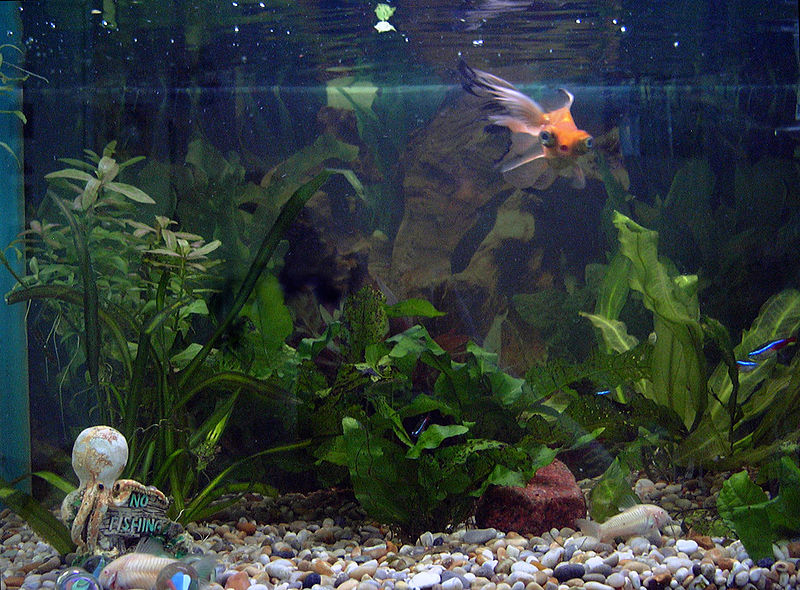
\includegraphics[width=6cm]{./imagenes/acuario2}}
\institute[LSE-FIUBA]{Laboratorio de Sistemas Embebidos - FIUBA\\ Ing. Patricio Bos}
\date{}

%\subtitle{Framework para aplicaciones de control de ambientes}
%\titlegraphic{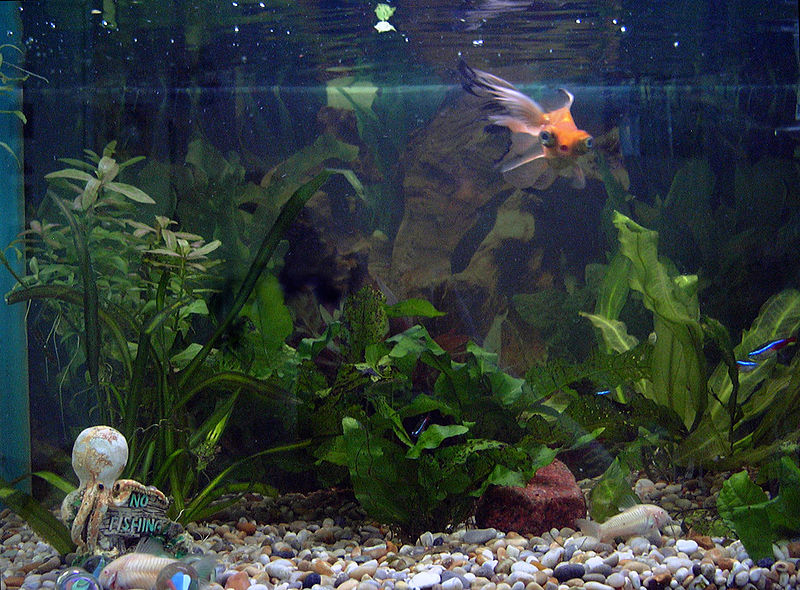
\includegraphics[width=5cm]{./imagenes/acuario2}}


\subject{Presentación del trabajo final de la Especialización en Sistemas Embebidos}
% This is only inserted into the PDF information catalog. Can be left
% out. 

\pgfdeclareimage[height=1.5cm]{university-logo}{./imagenes/logo-facu-inverso.png}
\logo{\pgfuseimage{university-logo}}


% If you wish to uncover everything in a step-wise fashion, uncomment
% the following command: 

\beamerdefaultoverlayspecification{<+->}
  
\begin{document}

%la magia del begingroup es para que titlepage quede centrada, sin eso queda
%corrida en el ancho del sidebar
\begingroup
\makeatletter
\setlength{\hoffset}{-.5\beamer@sidebarwidth}
\makeatother
\begin{frame}[plain,noframenumbering]
  \titlepage
\end{frame}

\endgroup



\begin{frame}{\textbf{Organización de la presentación}}
  \tableofcontents
  % You might wish to add the option [pausesections]
\end{frame}
%
%
%

\section{Motivación}

\begin{frame}{\textbf{¿Qué es un Acuario?}}
\fontsize{14pt}{15}\selectfont
\begin{minipage}[c]{1.0\linewidth}
\begin{minipage}[c]{0.6\linewidth}
	\begin{itemize}
		\item Ecosistema vivo y dinámico 
		% Recreación de un ambiente subacuático para albergar peces, invertebrados y plantas
		\vspace{10px}
		\item Interacciones complejas
		\vspace{10px}
		\item Uso recreativo o comercial
		\vspace{10px}
		\item Malas condiciones = \$
		\vspace{10px}
  	\end{itemize}	
  \end{minipage}
  \begin{minipage}[c]{0.35\linewidth}
	\begin{figure}[H]
		{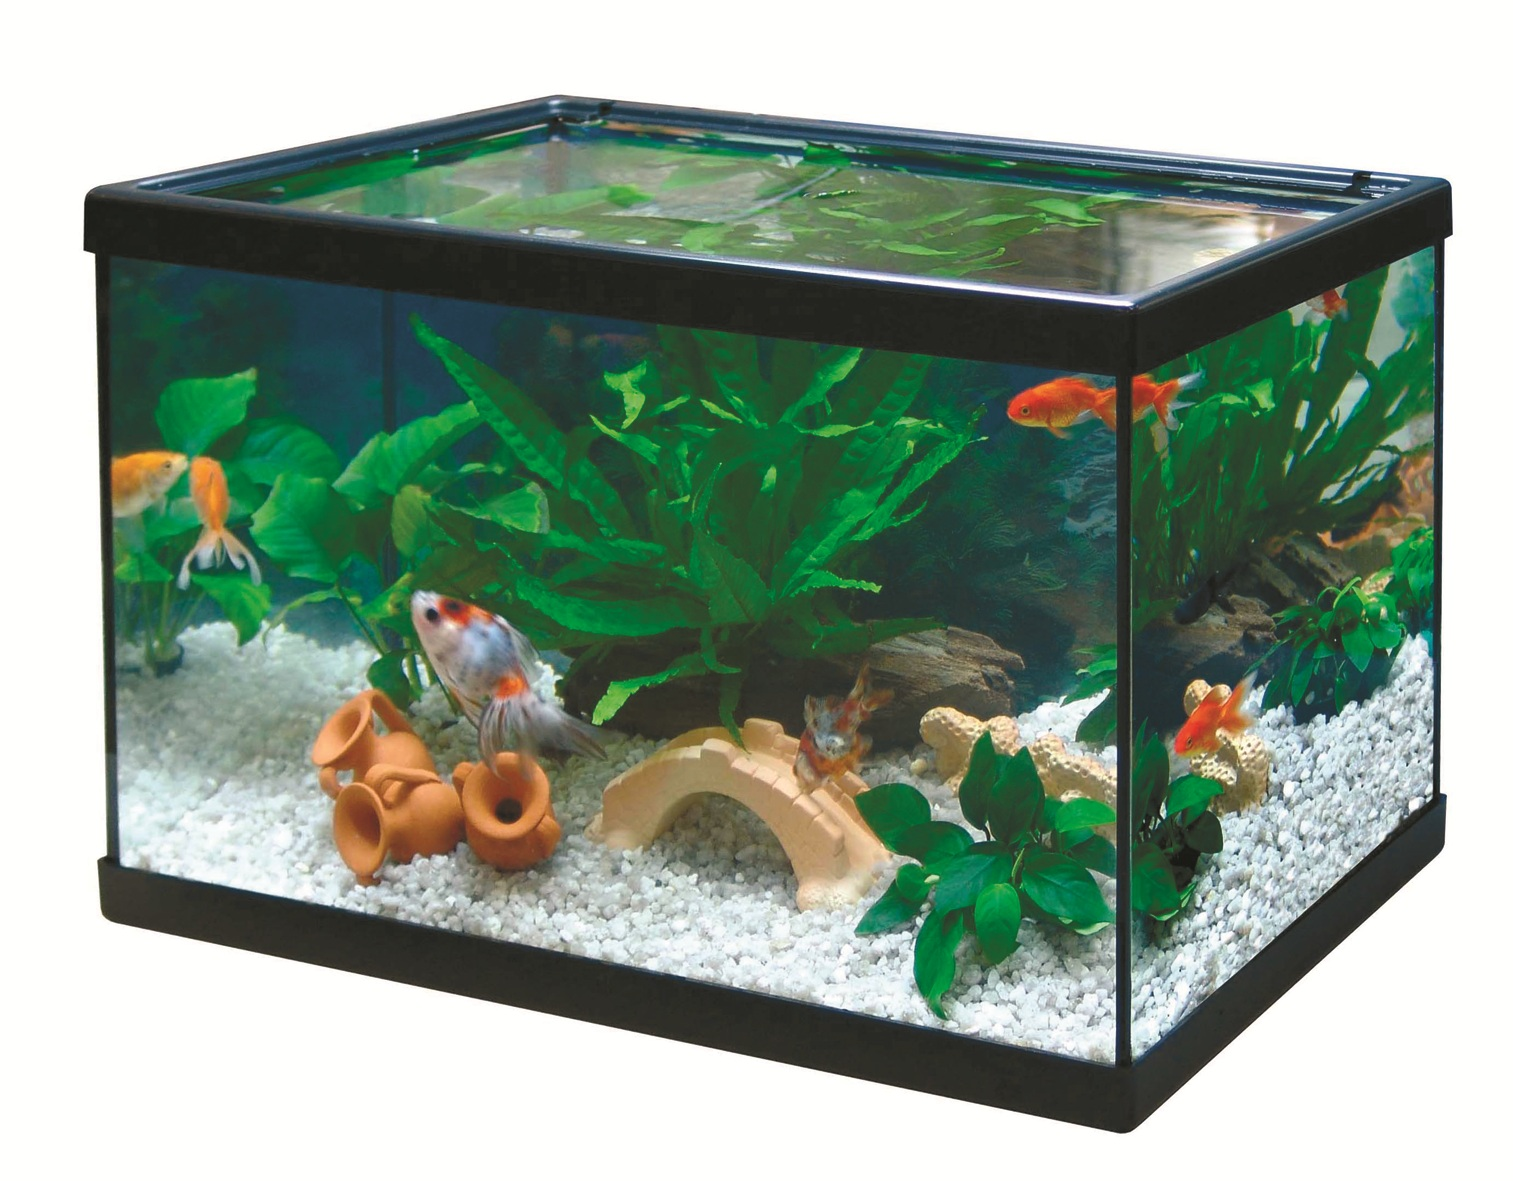
\includegraphics[width=1\textwidth]{./imagenes/acuario.jpg}}
	\end{figure}	  	  	
  \end{minipage}
\end{minipage}
\end{frame}

\begin{frame}{\textbf{Nemo así como lo ven...}}
\begin{align*}
	{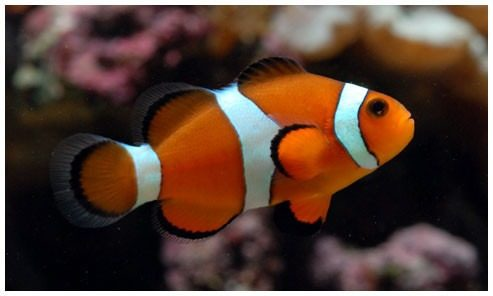
\includegraphics[width=1\textwidth]{./imagenes/nemo.jpg}}
\end{align*}


\end{frame}

\section[Problema]{Planteo del problema a resolver}

\begin{frame}{\textbf{Planteo del problema a resolver}}
\fontsize{18pt}{15}\selectfont
	\begin{itemize}
		\item {¿Qué hace falta medir?}
		\vspace{20px}
		\item ¿Qué hace falta controlar?
		\vspace{20px}
		\item ¿Sobre qué hace falta alertar?
		\vspace{10px}
	\end{itemize}
\end{frame}

\begin{frame}{\textbf{¿Qué hace falta medir? - Sensores}}
\fontsize{14pt}{15}\selectfont

\begin{minipage}[c]{1.0\linewidth}
\begin{minipage}[c]{0.6\linewidth}
      \centering
      \begin{itemize}
      	\item Temperatura
		\vspace{10px}
		\item pH
		\vspace{10px}
		\item Nivel de agua
		\vspace{10px}
		\item otros
			\begin{itemize}
				\item Conductividad
				\item Nitratos
				\item etc...
			\end{itemize}
	\end{itemize}
 \end{minipage}
  \begin{minipage}[c]{0.35\linewidth}
	\begin{figure}[H]
		{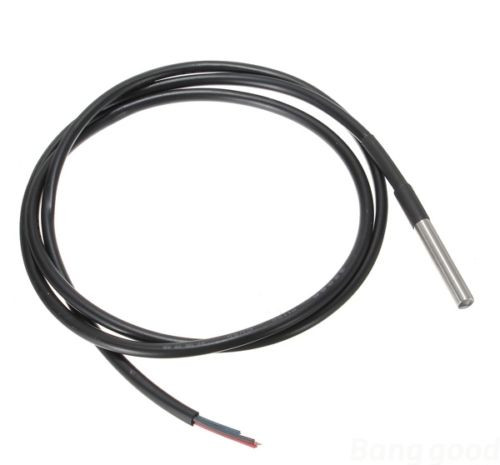
\includegraphics[width=1\textwidth]{./imagenes/sensor_temp}\vspace{5px}}
		{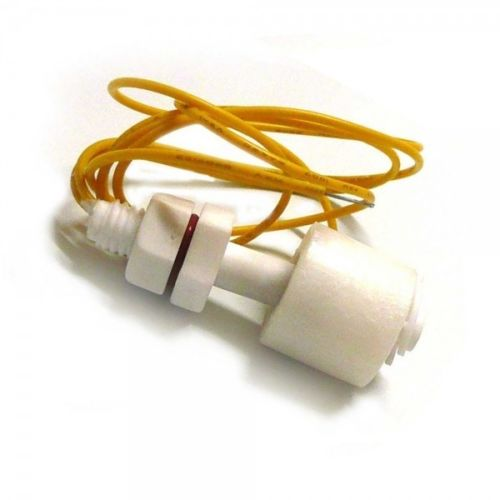
\includegraphics[width=1\textwidth]{./imagenes/sensor_nivel}}	
	\end{figure}	  	  	
  \end{minipage}
\end{minipage}
\end{frame}
	

\begin{frame}{\textbf{¿Qué hace falta controlar? - Actuadores}}
\fontsize{14pt}{15}\selectfont
\begin{minipage}[c]{1.0\linewidth}
\begin{minipage}[c]{0.6\linewidth}
      \centering
	\begin{itemize}
		\item Inyección de $O_2$/$CO_2$
		\vspace{10px}
		\item Iluminación
		\vspace{10px}
		\item Recambio de agua
		\vspace{10px}
		\item Calentadores
		\vspace{10px}
		\item Otros
			\begin{itemize}
				\item Dosificadores de alimento/nutrientes
				\item Refrigeración
				\item etc...
			\end{itemize}
	\end{itemize}
 \end{minipage}
  \begin{minipage}[c]{0.35\linewidth}
	\begin{figure}[H]
		{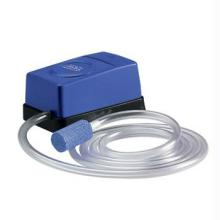
\includegraphics[width=1\textwidth]{./imagenes/actuador_pump}\vspace{5px}}
		{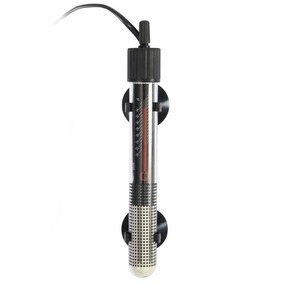
\includegraphics[width=1\textwidth]{./imagenes/actuador_heater}}	
	\end{figure}	  	  	
  \end{minipage}
\end{minipage}
\end{frame}

\begin{frame}{\textbf{¿Sobre qué hace falta alertar? - Alarmas}}
\fontsize{14pt}{15}\selectfont
\begin{itemize}
	\item Aviso de tarea periódica de mantenimiento
	\vspace{10px}
	\item Nivel de agua bajo/alto en tanques auxiliares
	\vspace{10px}
	\item Parámetro fuera de rango
	\vspace{10px}
	\item Falla de sensor
	\vspace{10px}
	\item Otros	
\end{itemize}	
\end{frame}

\begin{frame}{\textbf{Soluciones existentes}}
\fontsize{14pt}{15}\selectfont
\vspace{-10px}
	\begin{figure}
	\begin{align*} 
		{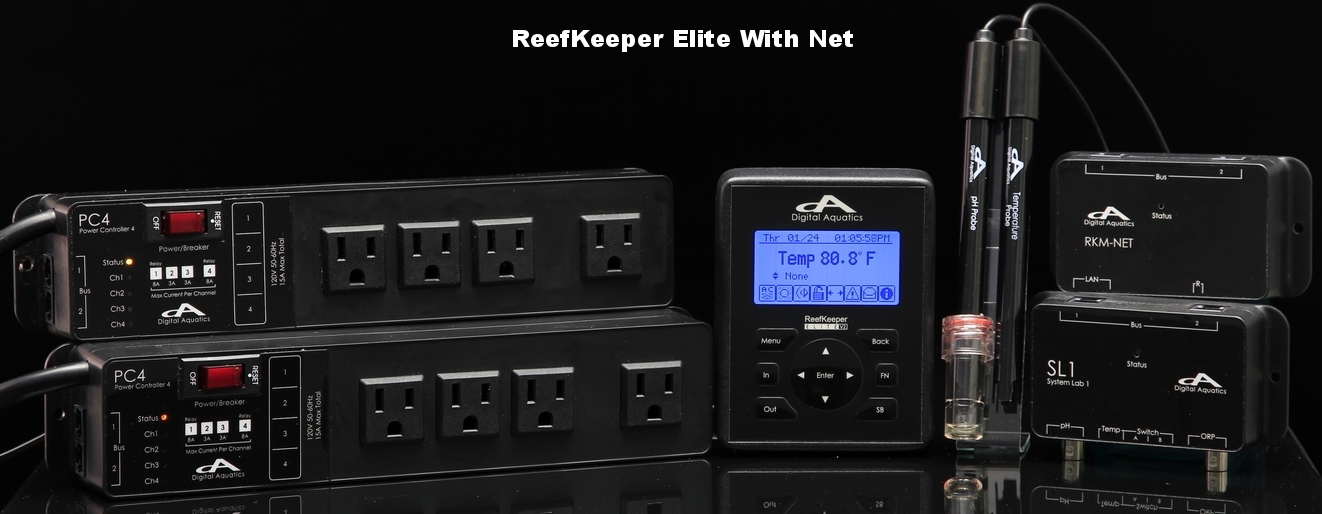
\includegraphics[width=.6\textwidth]{./imagenes/reefkeeper.JPG}}\\
		\vspace{15px}
		{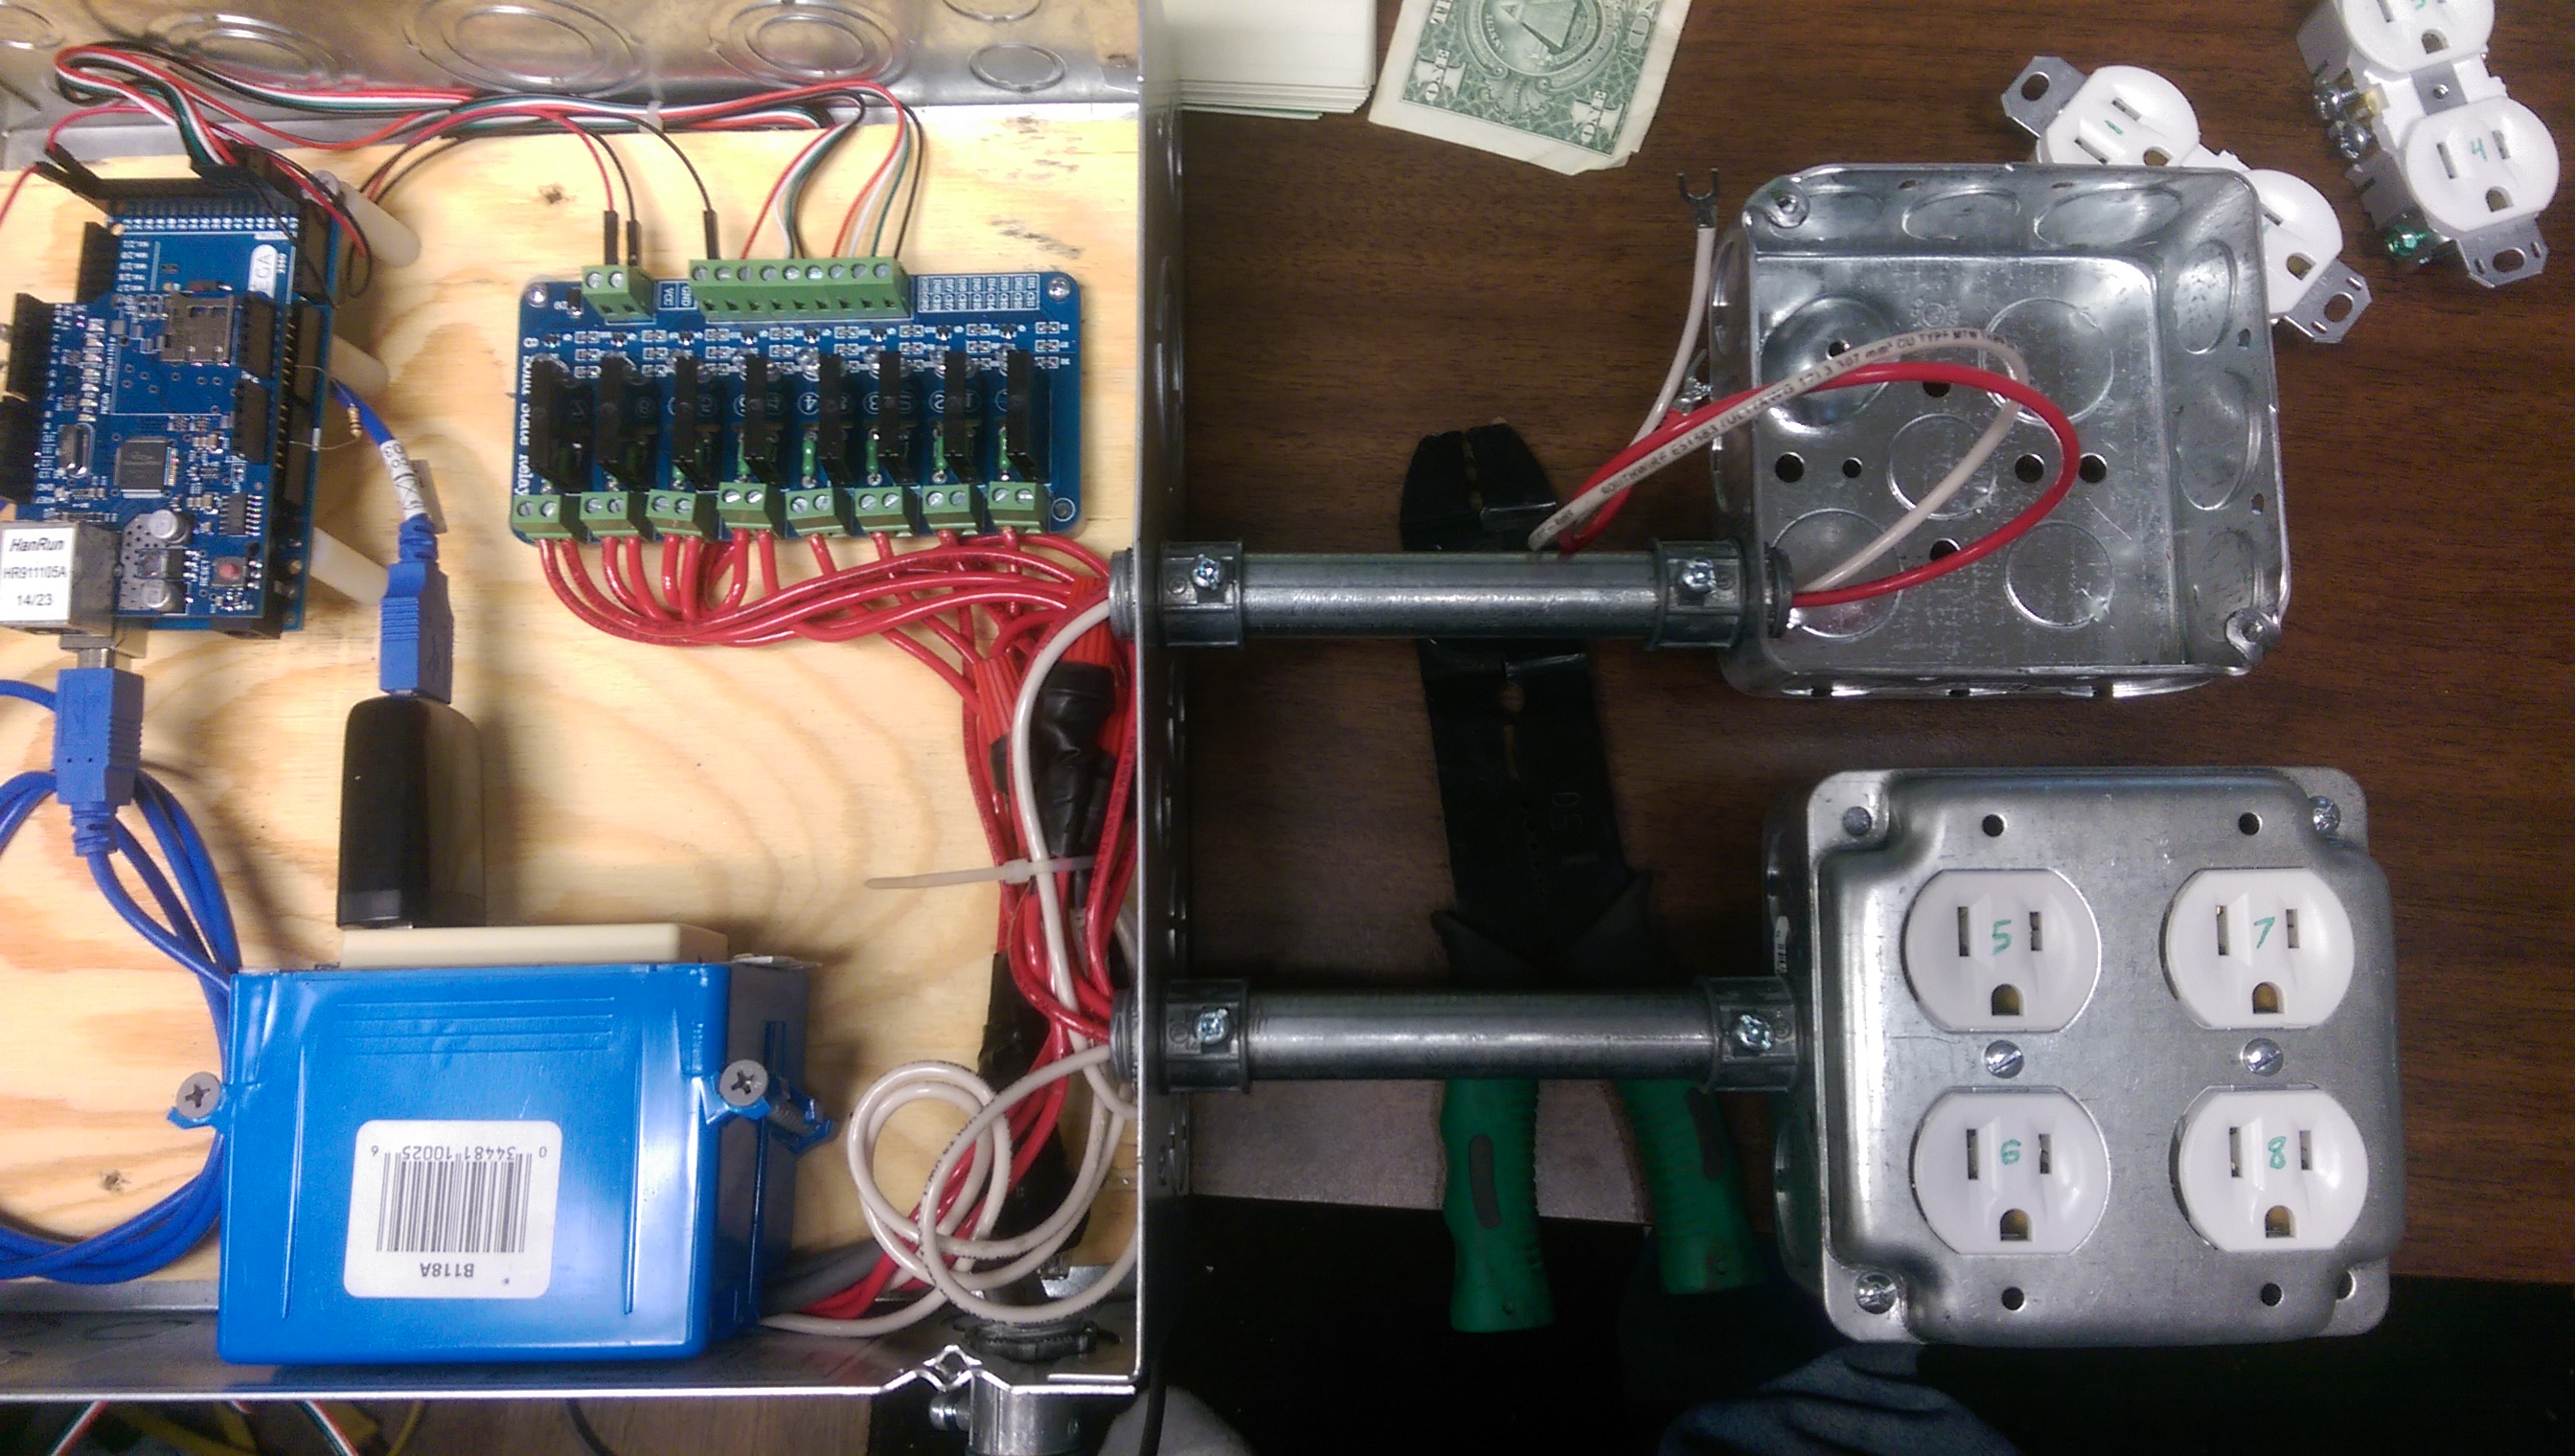
\includegraphics[width=.6\textwidth]{./imagenes/arduino.jpg}}
	\end{align*}
	\end{figure}	  	  	
\end{frame}
%



\section[Gestión]{Gestión de proyecto}
\subsection[Interesados]{Identificación de los Interesados}

\begin{frame}{\textbf{Identificación de los interesados}}
\fontsize{12pt}{15}\selectfont
\begin{itemize}
		\item \textbf{Cliente:} Dr. Ing. Ariel Lutemberg, director de la Carrera de Esp. en Sistemas Embebidos.
		\vspace{2px}
		\item \textbf{Sponsors:} LSE, Facultad de Ingeniería, UBA.
		\vspace{2px}
		\item \textbf{End Users:} Particulares / Tiendas / Productores.
		\vspace{2px}
		\item \textbf{Champion:} Dr. Ing. Ariel Lutemberg, Coordinador Proyecto CIAA.
		\vspace{2px}
		\item \textbf{Drivers:} Carolina González, Esteban de Mateo.
		\vspace{2px}
		\item \textbf{Supporters} Ing. Alejandro Celery
		\vspace{2px}
		\item \textbf{Project Manager:} Ing. Patricio Bos
		\vspace{2px}
		\item \textbf{Team Members:} Ing. Nicolás Moretti
	\end{itemize}
\end{frame}

\subsection[Scope]{Project Scope Statement}

\begin{frame}{\textbf{Project Scope Statement}}
\fontsize{14pt}{15}\selectfont
\begin{itemize}
\item \textbf{Objetivo:} Desarrollar un software que permita usar la CIAA como controlador de acuario.
\vspace{5px}
\item \textbf{Alcance:} Se limitan la cantidad de sensores, actuadores y alarmas.
\vspace{5px}
\item \textbf{Criterio de aceptación:} Visualizar en una interfaz web el estado del sistema y poder operar el conjunto de actuadores desde la misma interfaz.
\vspace{5px}
\item \textbf{Restricciones:} Finalizar el projecto antes del 15 de Diciembre de 2015.
\end{itemize}
\end{frame}

\subsection[WBS]{Work Breakdown Structure}

\begin{frame}{\textbf{WBS} Desglose de tareas}
\fontsize{14pt}{15}\selectfont
	\begin{enumerate}
		\item Gestión del projecto
		\vspace{10px}
		\item Hardware
		\vspace{10px}
		\item Firmware
		\vspace{10px}
		\item Interfaz web
		\vspace{10px}
		\item Verificación y Validación
		\vspace{10px}
	\end{enumerate}
\end{frame}


\begin{frame}{\textbf{WBS - 1}}
\fontsize{14pt}{15}\selectfont
\begin{figure}[H]
	  	{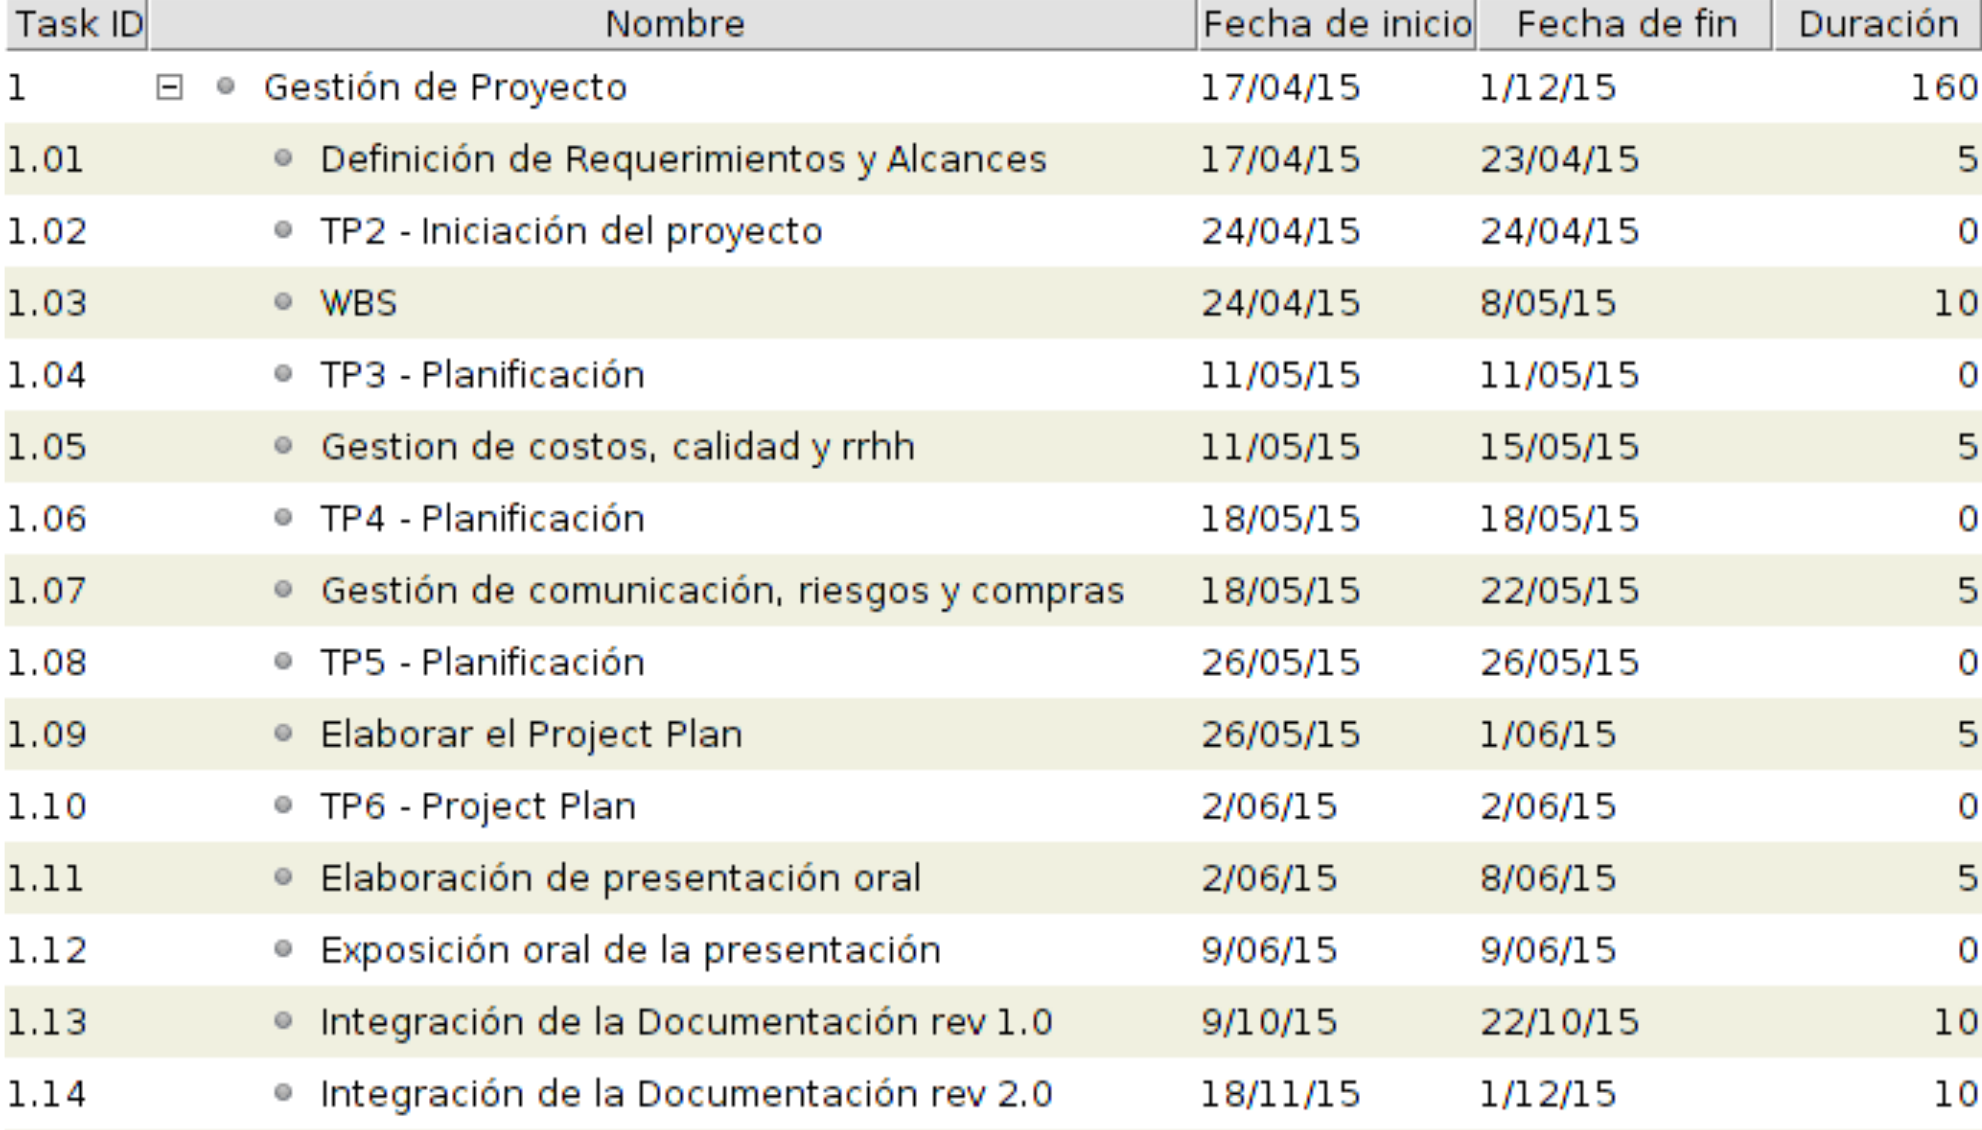
\includegraphics[width=1\textwidth]{./imagenes/wbs1.png}}
	\end{figure}	
\end{frame}

\begin{frame}{\textbf{WBS - 2}}
\fontsize{14pt}{15}\selectfont
\begin{figure}[H]
	  	{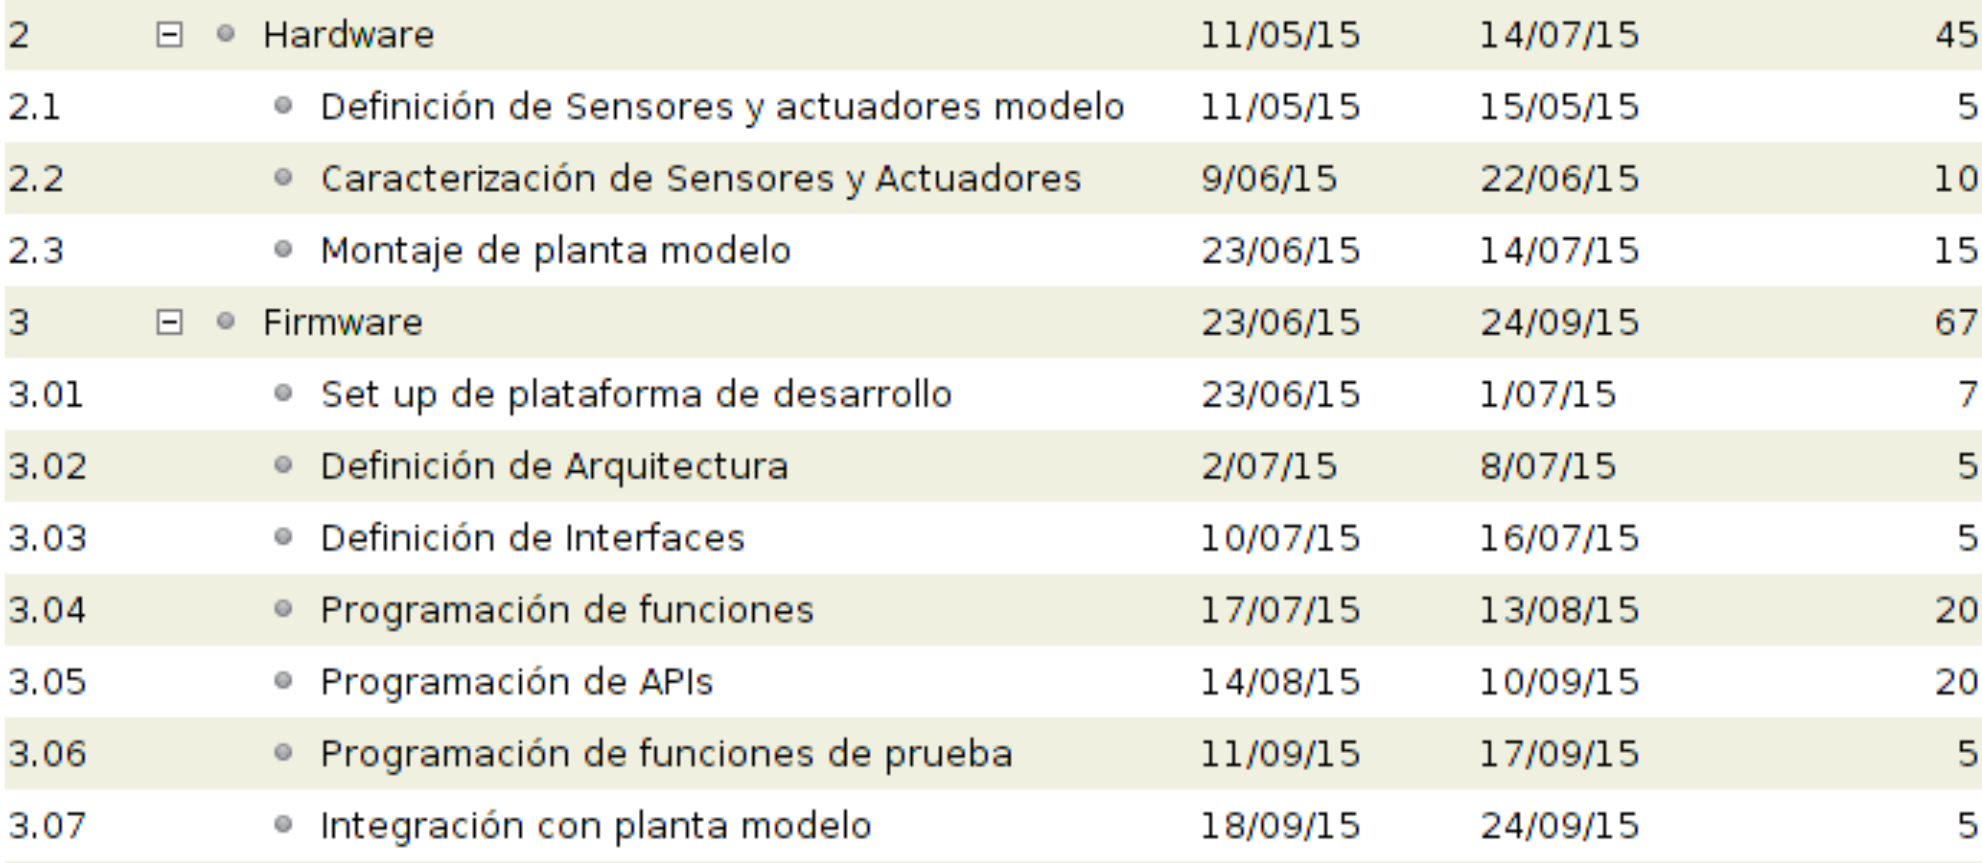
\includegraphics[width=1\textwidth]{./imagenes/wbs2.png}}
	\end{figure}	
\end{frame}


\begin{frame}{\textbf{WBS - 3}}
\fontsize{14pt}{15}\selectfont
\begin{figure}[H]
	  	{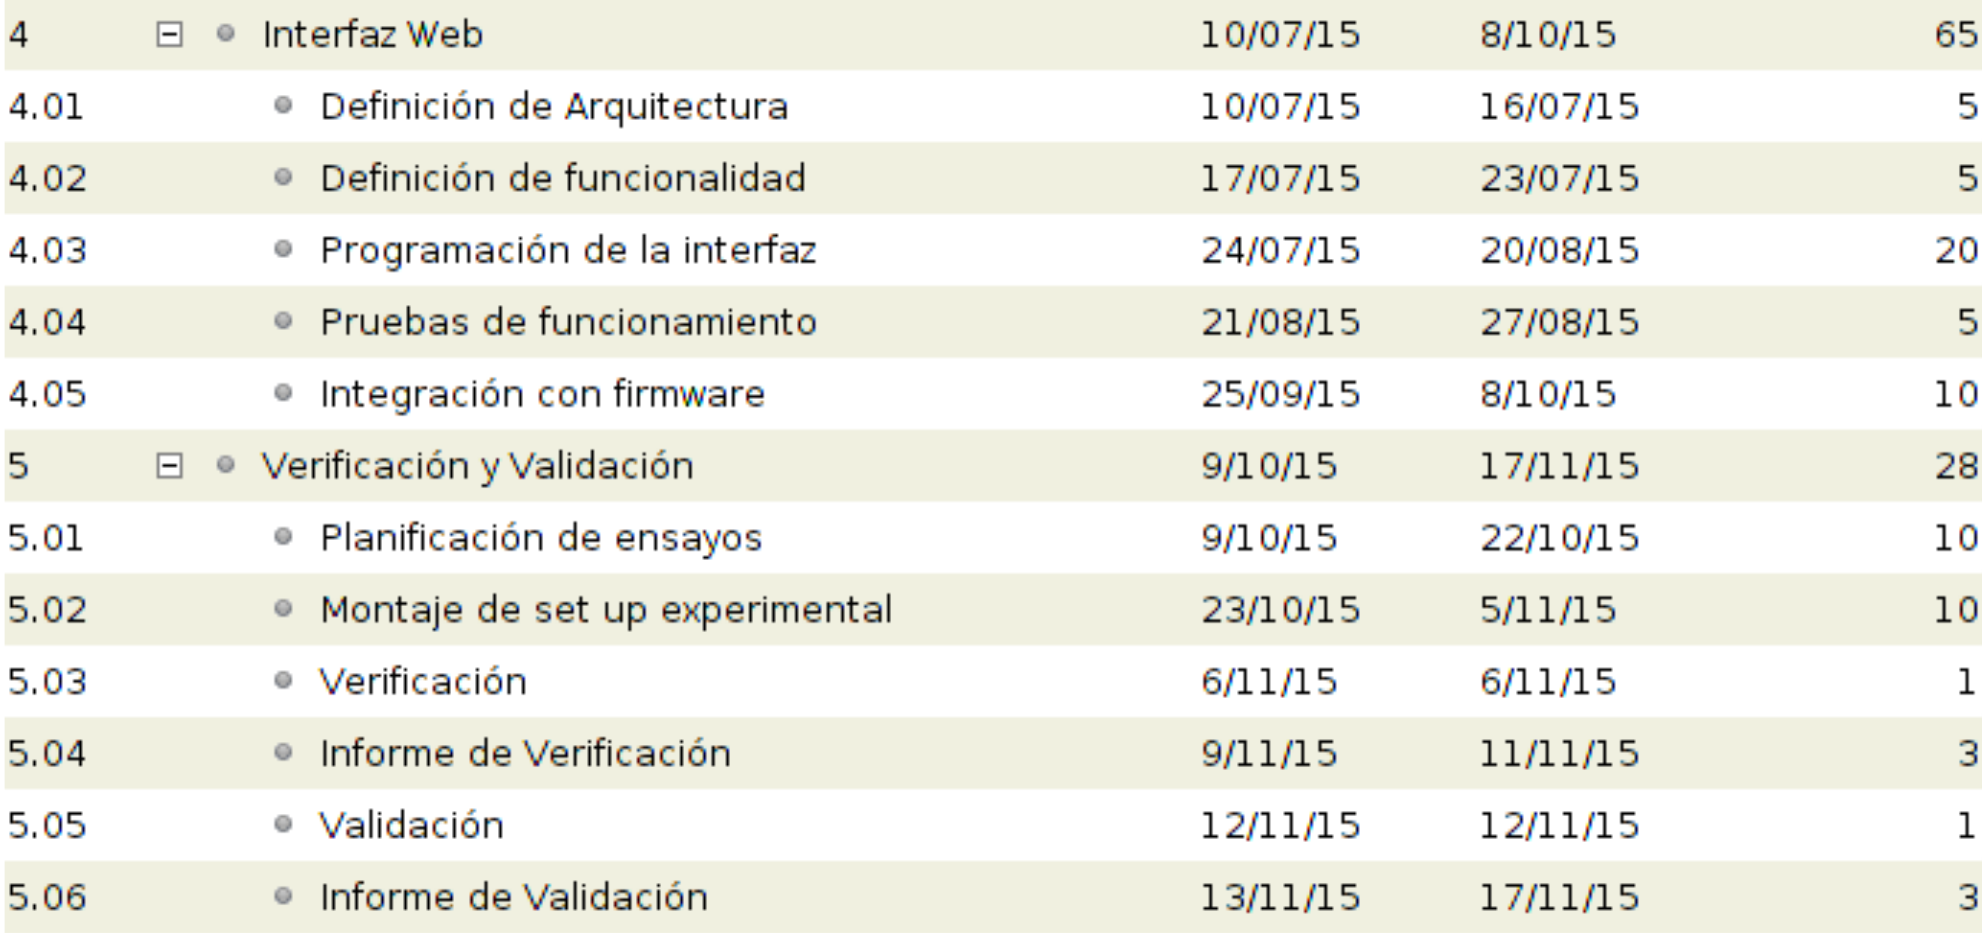
\includegraphics[width=1\textwidth]{./imagenes/wbs3.png}}
	\end{figure}	
\end{frame}



\begin{frame}{\textbf{Activity on Node}}
\fontsize{14pt}{15}\selectfont
	\begin{figure}[H]
	  	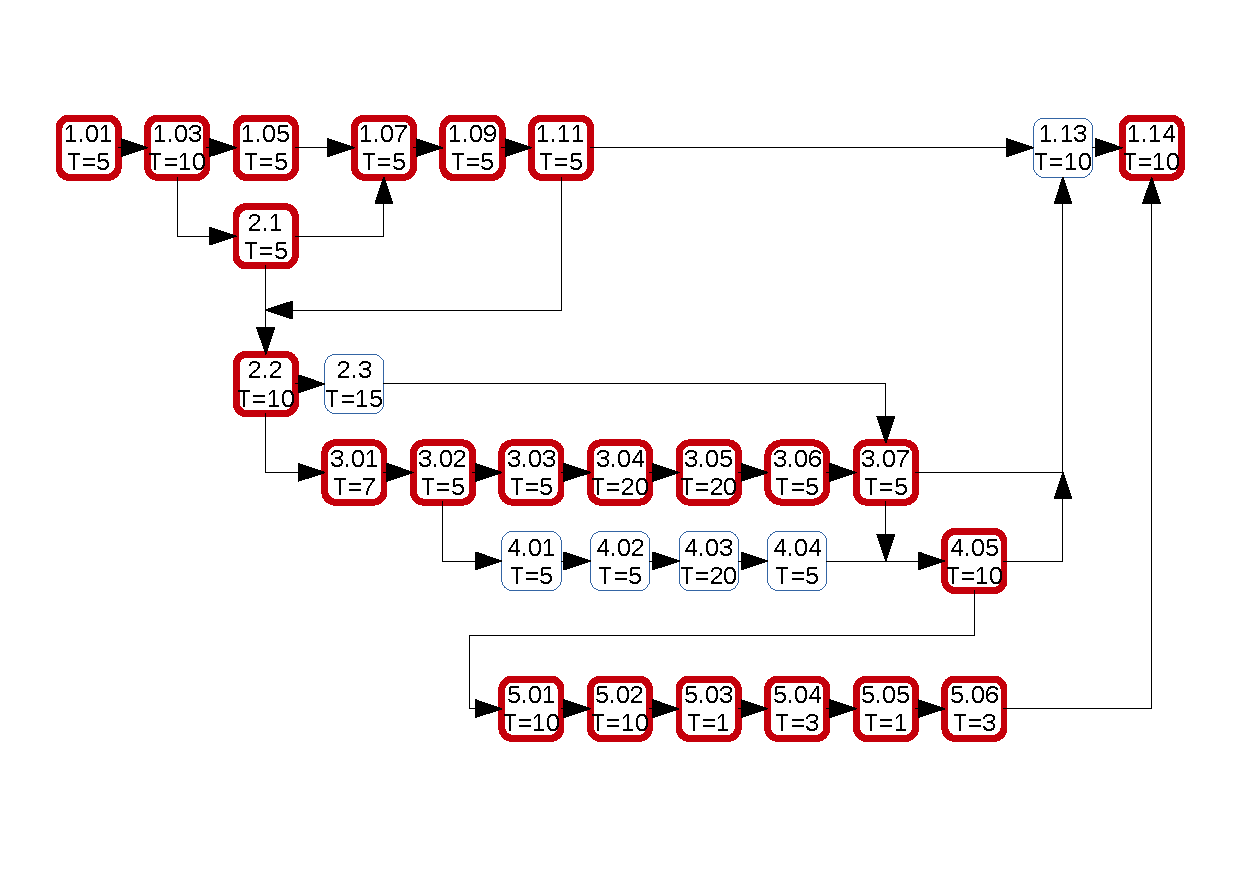
\includegraphics[width=1\textwidth]{./imagenes/AoN.pdf}
	\end{figure}	  
\end{frame}

\subsection[Calidad]{Gestión de Calidad}

\begin{frame}{\textbf{Gestión de Calidad}}
\fontsize{14pt}{15}\selectfont
	\begin{figure}[H]
	  	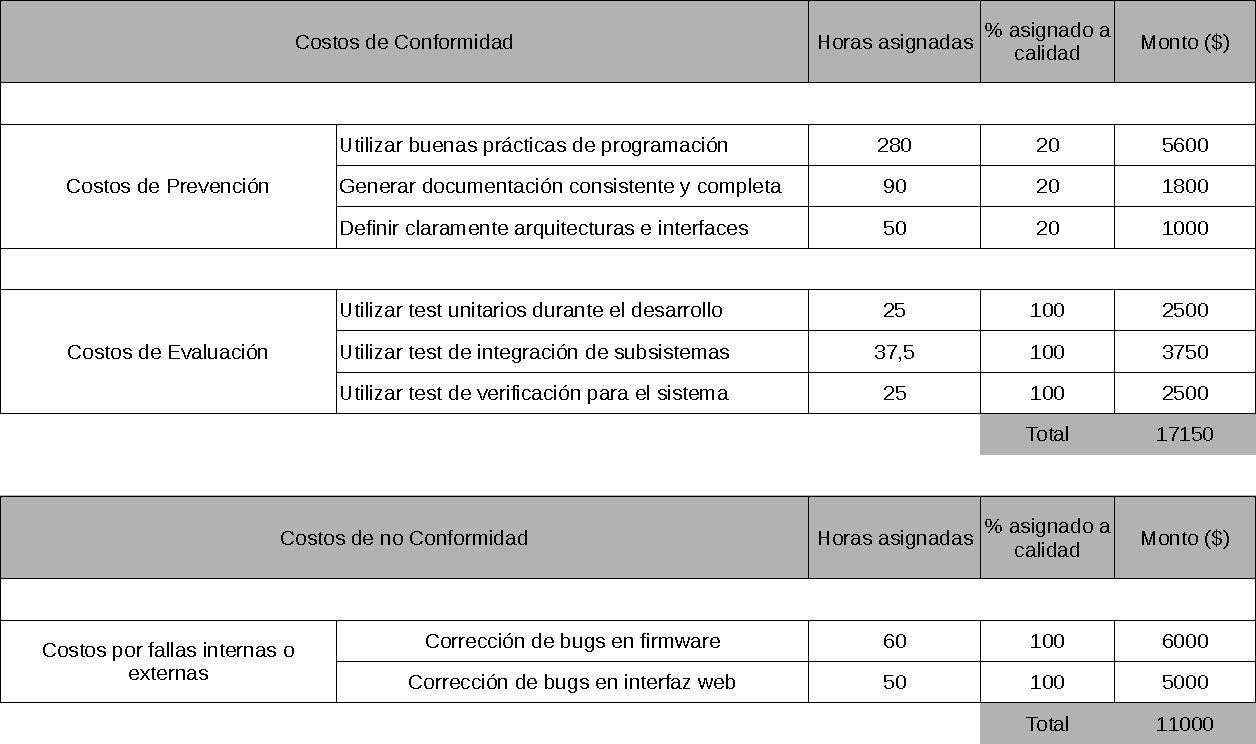
\includegraphics[width=1\textwidth]{./imagenes/tabla-calidad.pdf}
	\end{figure}	  
\end{frame}

\subsection[Recursos]{Gestión de Recursos}

\begin{frame}{\textbf{Gestión de Recursos y Costos}}
\fontsize{14pt}{15}\selectfont
	\begin{figure}[H]
	  	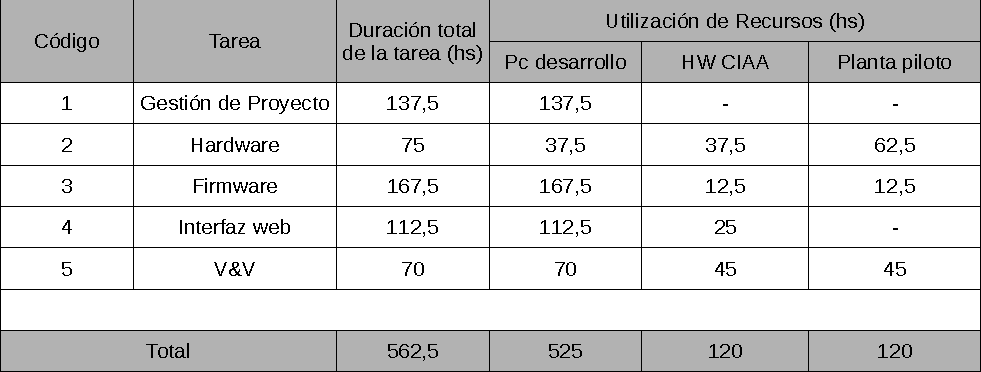
\includegraphics[width=1\textwidth]{./imagenes/tabla-recursos.pdf}\vspace{10px}
	  	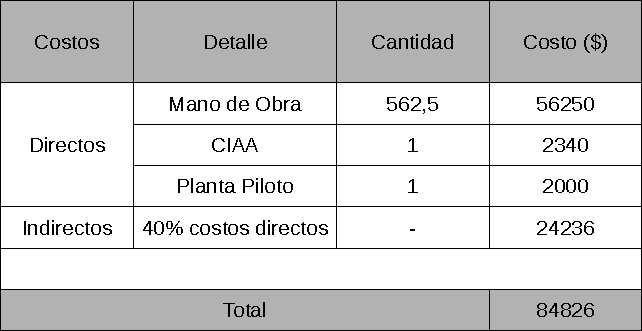
\includegraphics[width=.6\textwidth]{./imagenes/tabla-presupuesto.pdf}
	\end{figure}	  

\end{frame}

\subsection[Riesgos]{Gestión de Riesgos}

\begin{frame}{\textbf{Gestión de Riesgos}}
\fontsize{14pt}{15}\selectfont
	\begin{figure}[H]
	  	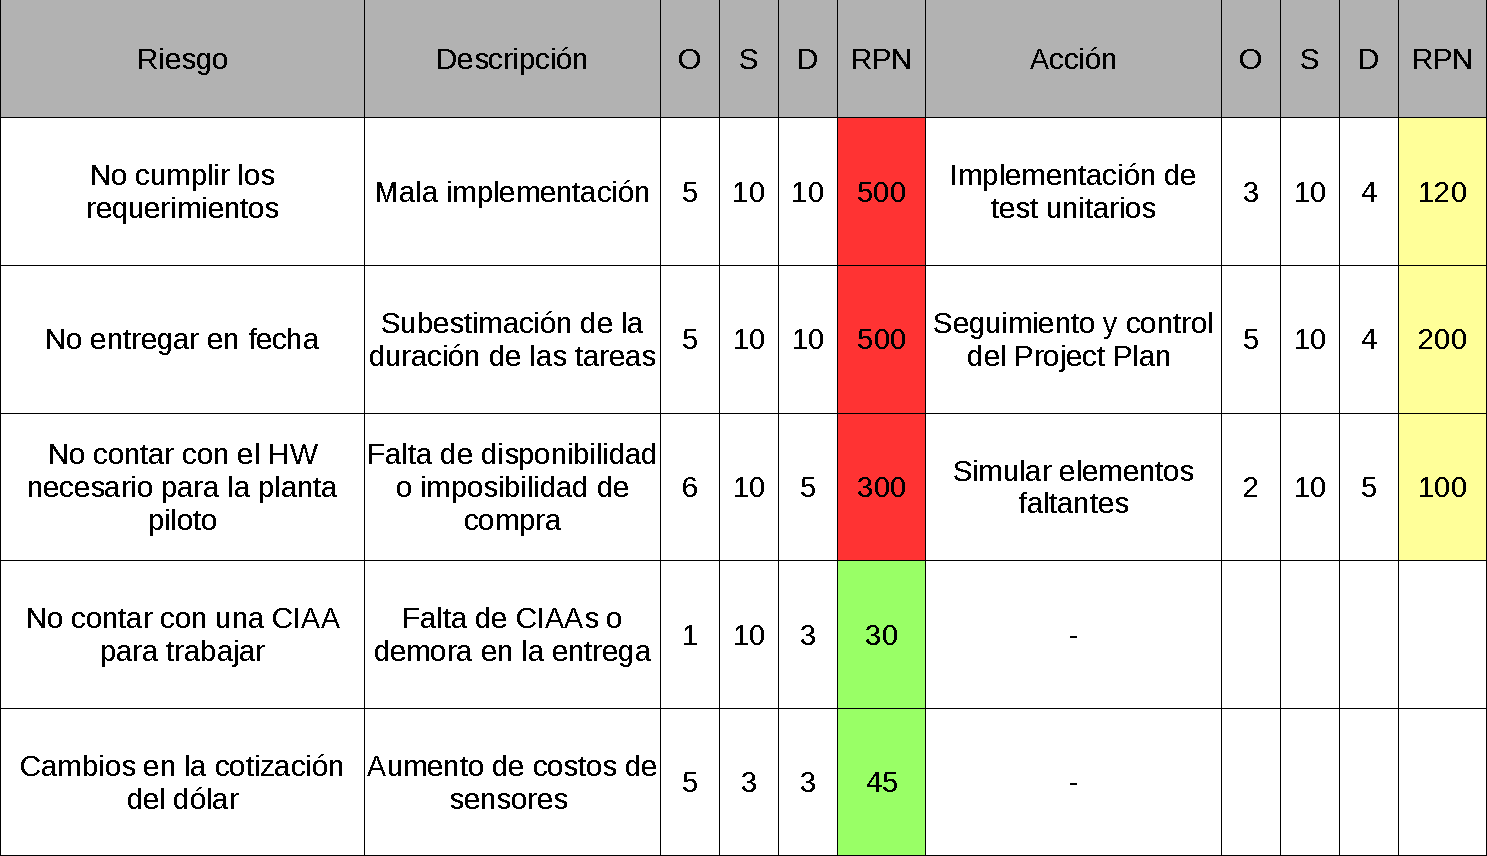
\includegraphics[width=1\textwidth]{./imagenes/tabla-riesgo.pdf}
	\end{figure}	  
\end{frame}


\begingroup
\makeatletter
\setlength{\hoffset}{-.5\beamer@sidebarwidth}
\makeatother
\begin{frame}[plain,noframenumbering]
\fontsize{18pt}{15}\selectfont
\begin{center}
	MUCHAS GRACIAS POR SU ATENCIÓN\\
	\vspace{2cm}
	¿PREGUNTAS?
\end{center}
\end{frame}
\endgroup

\end{document}